\documentclass[conference]{IEEEtran}
\IEEEoverridecommandlockouts
% The preceding line is only needed to identify funding in the first footnote. If that is unneeded, please comment it out.
\usepackage{tikz}
\usetikzlibrary{shapes.geometric, arrows}
\usetikzlibrary{arrows.meta,positioning}
\usepackage{float}
\usepackage{cite}
\usepackage{amsmath,amssymb,amsfonts}
\usepackage{algorithmic}
\usepackage{graphicx}
\usepackage{textcomp}
\usepackage{xcolor}
\graphicspath{ {./images/} }
\usepackage{multirow}

\usepackage{booktabs,tabularx}

\tikzstyle{startstop} = [rectangle, rounded corners, minimum width=3cm, minimum height=1cm,text centered, text width=3cm, draw=black, fill=white!30]
\tikzstyle{io} = [trapezium, trapezium left angle=70, trapezium right angle=110, minimum width=3cm, minimum height=1cm, text centered, text width=3cm, draw=black, fill=white!30]
\tikzstyle{process} = [rectangle, minimum width=4cm, minimum height=1cm, text centered,  text width=3cm, draw=black, fill=white!30]
\tikzstyle{decision} = [diamond, minimum width=3cm, minimum height=1cm, text centered, text width=3cm, draw=black, fill=white!30]
\tikzstyle{arrow} = [thick,->,>=stealth]

\def\BibTeX{{\rm B\kern-.05em{\sc i\kern-.025em b}\kern-.08em
		T\kern-.1667em\lower.7ex\hbox{E}\kern-.125emX}}
\begin{document}
	
	\title{Numerical Solution in Finding the Beam Deflection Caused by Small Free Vertical Vibrations Governed by Fourth-order Partial Differential Equation\\}
	
	\author{\IEEEauthorblockN{Eli Joshua V. Maravillas$^*$, Jhone Mychale Mariquit$^\dagger$}
		\IEEEauthorblockA{\textit{Department of Electrical Engineering and Technology}\\
			\textit{College of Engineering and Technology} \\
			\textit{Mindanao State University - Iligan Institute of Technology}\\
			Iligan City, Lanao del Norte, Philippines, 9200 \\
			$^*$elijoshua.maravillas@g.msuiit.edu.ph, $^\dagger$jhonemychale.mariquit@g.msuiit.edu.ph}
	}
	
	\maketitle
	
	\begin{IEEEkeywords}
		Fourth-order Partial Differential Equation, Fourth-order Partial Differential Equation derivation, Finite Difference Method with Matlab
	\end{IEEEkeywords}
	
	\section{Problem Statement}
	
	\begin{figure}[h]
		\centering
		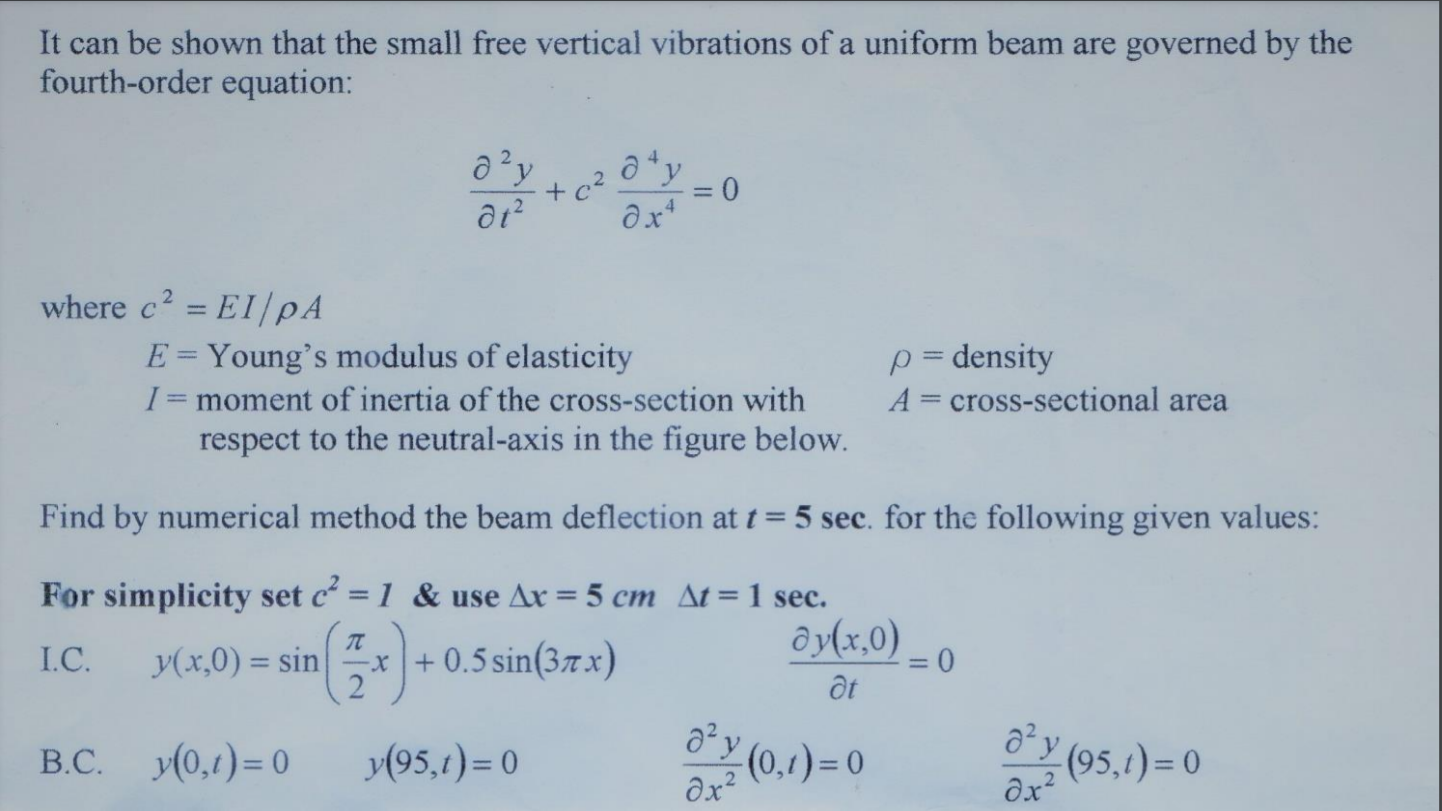
\includegraphics[width=0.45\textwidth]{1.png}
		\caption{Problem Statement}
	\end{figure}
	\begin{figure}[h]
		\centering
		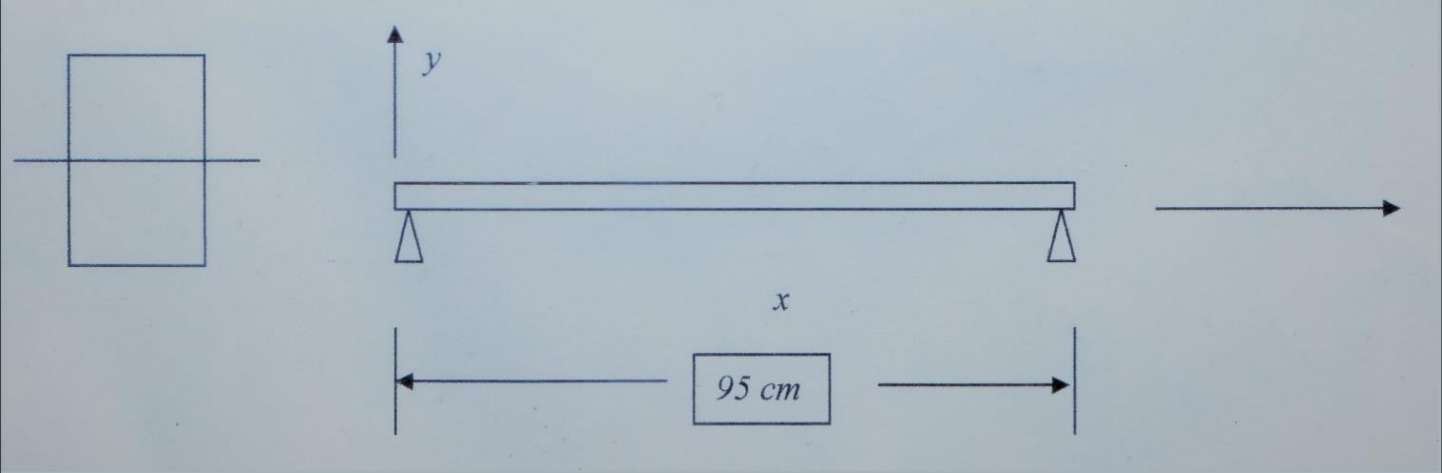
\includegraphics[width=0.45\textwidth]{2.png}
		\caption{Problem Diagram}
	\end{figure}
	
	The above problem can be solved using Finite Difference Method to formulate an algorithm based on the given partial differential equation by replacing the derivatives with algebraic equations. In this case, it should be established first the algebraic notation by:
	
	\begin{equation}
		\label{eqn: Notation1}
		y_{i},_{j} = 
		\begin{cases}
			i,&\ \text{temporal index for time t} \\
			j,&\ \text{spatial index for length x}
		\end{cases}
	\end{equation}

	For interval evaluation, the points can be checked by incrementing the indexes in each step as shown below
	\begin{equation}
		\label{eqn: Notation2}
		y_{i + Nt},_{j + Nx} = 
		\begin{cases}
			Nt,&\ \text{Nt is the total t interval} \\
			Nx,&\ \text{Nx is the total x interval}
		\end{cases}
	\end{equation}

	Derivatives can also be looked as the slope of the line between two points. It can also be simplified as the rise divided by the run between two points where
	
	\begin{equation}
		\label{eqn: Derivative}
		\frac{\partial y}{\partial x} = \frac{\bigtriangleup y}{\bigtriangleup x}
		\begin{cases}
			\bigtriangleup y,&\ \text{the interval in y} \\
			\bigtriangleup x,&\ \text{the interval in x}
		\end{cases}
	\end{equation}
	\begin{equation}
		\label{eqn: Derivative2}
		\frac{\partial y}{\partial x} = \frac{y(x + \bigtriangleup x) - y(x - \bigtriangleup x)}{2\bigtriangleup x}
	\end{equation}
	
	or can be simplified as 
	\begin{equation}
		%\ref{eqn: Derivative2}
		\label{eqn: Derivative3}
		\frac{\partial y}{\partial x} = \frac{y(x + \bigtriangleup x)}{\bigtriangleup x}
		%\ref{eqn: Derivative2}
	\end{equation}
	
	If we let
	\begin{equation}
		%\label{eqn: Derivative}
		h,g = 
		\begin{cases}
			h = \bigtriangleup t\\
			g = \bigtriangleup x
		\end{cases}
	\end{equation}
	and substituting equation \eqref{eqn: Notation1} and equation \eqref{eqn: Derivative} to equation \eqref{eqn: Derivative2}, we get
	\begin{equation}
		%\ref{eqn: Derivative2}
		\label{eqn: Derivative6}
		\frac{\bigtriangleup y}{\bigtriangleup t} = \frac{y_{i},_{j} - y_{i-1},_{j}}{h}
		%\ref{eqn: Derivative2}
	\end{equation}

	\begin{equation}
		%\ref{eqn: Derivative7}
		\label{eqn: Derivative7}
		\frac{\bigtriangleup y}{\bigtriangleup x} = \frac{y_{i},_{j} - y_{i},_{j-1}}{h}
		%\ref{eqn: Derivative2}
	\end{equation}
	
	\section{Derivation}
	\subsection{Central Difference Method}
	We can now derive the needed algebraic equations to solve the fourth-order partial differential equations. 
	From equation \eqref{eqn: Derivative6} and equation \eqref{eqn: Derivative7}, we can further dive down into higher order derivatives by using Central Difference Method. For second order derivative we can further derive \eqref{eqn: Derivative2} to,
	
	
	\begin{equation}
		%\ref{eqn: Derivative2}
		\label{eqn: Derivative8}
		\frac{\bigtriangleup^2 y}{\bigtriangleup t^2} =\frac{1}{h}\left[\frac{y_{i+1},_{j} - y_{i},_{j}}{h} - \frac{y_{i},_{j} - y_{i-1},_{j}}{h} \right]
		%\ref{eqn: Derivative2}
	\end{equation}
	
	\begin{equation}
		%\ref{eqn: Derivative2}
		\label{eqn: Derivative9}
		\frac{\bigtriangleup^2 y}{\bigtriangleup t^2} =\frac{1}{h^2}\left[{y_{i+1},_{j} - 2 y_{i},_{j} + y_{i-1},_{j}} \right]
		%\ref{eqn: Derivative2}
	\end{equation}
	
	and 
	\begin{equation}
		%\ref{eqn: Derivative2}
		\label{eqn: Derivative10}
		\frac{\bigtriangleup^2 y}{\bigtriangleup x^2} =\frac{1}{g^2}\left[{y_{i},_{j+1} - 2 y_{i},_{j} + y_{i},_{j-1}} \right]
		%\ref{eqn: Derivative2}
	\end{equation}
	
	For the third-order derivative, we can further derive equations \eqref{eqn: Derivative9} and \eqref{eqn: Derivative10} to
	
	\begin{align}
		\label{eqn: Derivative11}
		\frac{\bigtriangleup^3 y}{\bigtriangleup t^3} = \frac{1}{h} &\left[\frac{y_{i+2},_{j} - 2 y_{i+1},_{j} + y_{i},_{j}}{h^2}\right]\\
		&-\frac{1}{h}\left[\frac{y_{i-1},_{j} - 2 y_{i},_{j} + y_{i-1},_{j}}{h^2}\right]\notag
	\end{align}
	
	simplifying equation \eqref{eqn: Derivative12} we get
	\begin{equation}
		%\ref{eqn: Derivative2}
		\label{eqn: Derivative12}
		\frac{\bigtriangleup^3 y}{\bigtriangleup t^3} =\left[\frac{y_{i+2},_{j} - 3 y_{i+1},_{j} - 3 y_{i},_{j} - y_{i-1},_{j}}{h^3}\right]
		%\ref{eqn: Derivative2}
	\end{equation}
	
	and 
	
	\begin{equation}
		%\ref{eqn: Derivative2}
		\label{eqn: Derivative13}
		\frac{\bigtriangleup^3 y}{\bigtriangleup g^3} =\left[\frac{y_{i},_{j+2} - 3 y_{i},_{j+1} - 3 y_{i},_{j} - y_{i},_{j-1}}{g^3}\right]
		%\ref{eqn: Derivative2}
	\end{equation}

	For the fourth-order derivative, we can further derive equations \eqref{eqn: Derivative12} and \eqref{eqn: Derivative13} to
	
	\begin{align}
		\label{eqn: Derivative14}
		\frac{\bigtriangleup^4 y}{\bigtriangleup t^4} = \frac{1}{h} &\left[\frac{y_{i+3},_{j} - 3 y_{i+2},_{j} - 3 y_{i+1},_{j} - y_{i},_{j}}{h^3}\right]\\
		&-\frac{1}{h}\left[\frac{y_{i+2},_{j} - 3 y_{i+1},_{j} - 3 y_{i},_{j} - y_{i-1},_{j}}{h^3}\right]\notag
	\end{align}

	simplifying equation \eqref{eqn: Derivative14} we get
	\begin{equation}
		%\ref{eqn: Derivative2}
		\label{eqn: Derivative15}
		\frac{\bigtriangleup^4 y}{\bigtriangleup t^4} =\left[\frac{y_{i+2},_{j} - 4 y_{i+1},_{j} + 6 y_{i},_{j} - 4 y_{i-1},_{j} + y_{i-1},_{j}}{h^4} \right]
		%\ref{eqn: Derivative2}
	\end{equation}

	and 
	\begin{equation}
		%\ref{eqn: Derivative2}
		\label{eqn: Derivative16}
		\frac{\bigtriangleup^4 y}{\bigtriangleup g^4} =\left[\frac{y_{i+2},_{j} - 4 y_{i+1},_{j} + 6 y_{i},_{j} - 4 y_{i-1},_{j} + y_{i-1},_{j}}{g^4} \right]
		%\ref{eqn: Derivative2}
	\end{equation}

	\subsection{Finding the general equation of the algorithm}
	The given equation in the problem statement, given by 
	
	\begin{equation}
		%\ref{eqn: Derivative2}
		\label{eqn: Derivative17}
		\frac{\partial^2 y}{\partial t^2}  + c^2 \frac{\partial^4 y}{\partial^4 x} = 0
		%\ref{eqn: Derivative2}
	\end{equation}
	
	simplifying equation \eqref{eqn: Derivative17} we get
	
	\begin{equation}
		%\ref{eqn: Derivative2}
		\label{eqn: Derivative18}
		\frac{\partial^2 y}{\partial t^2}  = - c^2 \frac{\partial^4 y}{\partial^4 x}
		%\ref{eqn: Derivative2}
	\end{equation}

	Substituting equations \eqref{eqn: Derivative9} and \eqref{eqn: Derivative16} to equation \eqref{eqn: Derivative18} we get
	
	\begin{align}
		\label{eqn: Derivative19}
		&\frac{1}{h^2}\left[{y_{i+1},_{j} - 2 y_{i},_{j} + y_{i-1},_{j}}\right]&\\
		&= - \frac{1}{g^4}\left[{y_{i+2},_{j} - 4 y_{i+1},_{j} + 6 y_{i},_{j} - 4 y_{i-1},_{j} + y_{i-1},_{j}} \right]\notag
	\end{align}\\
	
	Simplifying equation \eqref{eqn: Derivative19} extracting \begin{math}y_{i+1},_{j}\end{math} , we get
	
	\begin{align}
		\label{eqn: Derivative20}
		y_{i+1},_{j} = 
		-\frac{h^2}{g^4}\left[ Yx\right] + 2 y_{i},_{j} - y_{i-1},_{j}
	\end{align}
	where 
	\begin{equation}
		%\ref{eqn: Derivative2}
		\label{eqn: Derivative21}
		Yx  = {y_{i+2},_{j} - 4 y_{i+1},_{j} + 6 y_{i},_{j} - 4 y_{i-1},_{j} + y_{i-1},_{j}}
		%\ref{eqn: Derivative2}
	\end{equation}

	Equation \eqref{eqn: Derivative21} would then be our general equation in solving this problem.
	
	\subsection{Solving Initial Conditions and Boundary Conditions}
	
	Given initial conditions,
	\begin{equation}
		%\ref{eqn: Derivative2}
		\label{eqn: Derivative22}
		y(0,x)  = sin(\frac{\pi}{2} x) + 0.5 sin (3\pi x)
		%\ref{eqn: Derivative2}
	\end{equation} 
	using equation \eqref{eqn: Derivative22} we can solve for the beam deflection at time 0 sec. However, the derived general equation \eqref{eqn: Derivative21}, this involves a set of data which is beyond the boundaries of the problem, at time equals -1 sec. In order to solve this, we need to look for new set of rules from our initial and boundary conditions.
	
	From the given initial condition, 
	
	\begin{equation}
		%\ref{eqn: Derivative2}
		\label{eqn: Derivative23}
		\frac{\partial y(0,x)}{\partial t}  = 0
		%\ref{eqn: Derivative2}
	\end{equation} 
	
	we can evaluate the initial condition in the form similar to equation \eqref{eqn: Derivative7}, in which we can simplify to get a new condition. Plugging in equation \eqref{eqn: Derivative23} to equation \eqref{eqn: Derivative7}, we get
	
	\begin{equation}
		%\ref{eqn: Derivative2}
		\label{eqn: Derivative24}
		\frac{y_{i},_{j} - y_{i},_{j-1}}{h}  = 0
		%\ref{eqn: Derivative2}
	\end{equation} 

	Simplifying equation \eqref{eqn: Derivative24}, we get 
	
	\begin{equation}
		%\ref{eqn: Derivative2}
		\label{eqn: Derivative25}
		{y_{i},_{j} = y_{i},_{j-1}, t = 0}  
		%\ref{eqn: Derivative2}
	\end{equation} 
	We can use equation \eqref{eqn: Derivative25} in getting new values from the derived general equation \eqref{eqn: Derivative20}.
	
	Solving for the boundary conditions can be derived from the given boundary condition equations
	
	\begin{equation}
		%\ref{eqn: Derivative2}
		\label{eqn: Derivative26}
		{y(t,0) = 0}
		%\ref{eqn: Derivative2}
	\end{equation} 
	\begin{equation}
		%\ref{eqn: Derivative2}
		\label{eqn: Derivative27}
		{y(t,95) = 0}
		%\ref{eqn: Derivative2}
	\end{equation} 
	\begin{equation}
		%\ref{eqn: Derivative2}
		\label{eqn: Derivative28}
		\frac{\partial^2 y(t,0)}{\partial x^2}  = 0
		%\ref{eqn: Derivative2}
	\end{equation} 
	\begin{equation}
		%\ref{eqn: Derivative2}
		\label{eqn: Derivative29}
		\frac{\partial^2 y(t,95)}{\partial x^2}  = 0
		%\ref{eqn: Derivative2}
	\end{equation} 
	From equations \eqref{eqn: Derivative26} to \eqref{eqn: Derivative29}, we can get the boundary equations equal to
	
	\begin{equation}
		%\ref{eqn: Derivative2}
		\label{eqn: Derivative30}
		{y_{i},_{1} = - y_{i},_{-1}, x = 0}  
		%\ref{eqn: Derivative2}
	\end{equation}  
	and
	
	\begin{equation}
		%\ref{eqn: Derivative2}
		\label{eqn: Derivative31}
		{y_{i},_{20} = - y_{i},_{18}, x = 95}  
		%\ref{eqn: Derivative2}
	\end{equation}  

	\subsection{Final General Equation}
	
	The general equation derived from the Finite Difference method would then be 
	
	\begin{align}
		\label{eqn: Derivative32}
		y_{i+1},_{j} = 
		-\frac{h^2}{g^4}\left[ Yx\right] + 2 y_{i},_{j} - y_{i-1},_{j}
	\end{align}
	where 
	\begin{equation}
		%\ref{eqn: Derivative2}
		\label{eqn: Derivative33}
		Yx  = {y_{i+2},_{j} - 4 y_{i+1},_{j} + 6 y_{i},_{j} - 4 y_{i-1},_{j} + y_{i-1},_{j}}
		%\ref{eqn: Derivative2}
	\end{equation}
	with initial conditions 
	\begin{equation}
		%\ref{eqn: Derivative2}
		\label{eqn: Derivative34}
		y(0,x)  = sin(\frac{\pi}{2} x) + 0.5 sin (3\pi x)
		%\ref{eqn: Derivative2}
	\end{equation} 
	\begin{equation}
		%\ref{eqn: Derivative2}
		\label{eqn: Derivative35}
		{y_{i},_{j} = y_{i},_{j-1}, t = 0}  
		%\ref{eqn: Derivative2}
	\end{equation} 
	and	boundary conditions
	\begin{equation}
		%\ref{eqn: Derivative2}
		\label{eqn: Derivative36}
		{y(t,0) = 0}
		%\ref{eqn: Derivative2}
	\end{equation} 
	\begin{equation}
		%\ref{eqn: Derivative2}
		\label{eqn: Derivative37}
		{y(t,95) = 0}
		%\ref{eqn: Derivative2}
	\end{equation} 
	\begin{equation}
		%\ref{eqn: Derivative2}
		\label{eqn: Derivative38}
		{y_{i},_{1} = - y_{i},_{-1}, x = 0}  
		%\ref{eqn: Derivative2}
	\end{equation}  

	\begin{equation}
		%\ref{eqn: Derivative2}
		\label{eqn: Derivative39}
		{y_{i},_{20} = - y_{i},_{18}, x = 95}  
		%\ref{eqn: Derivative2}
	\end{equation}  
\end{document}
